\documentclass[notas.tex]{subfiles} 				%tamanho das paginas: a4

\begin{document}
\section{Geometry dependence of quantum Hall wave functions} \label{sec_geometry_dependence}

\subsection{Dynamics of a particle on a magnetic field} \label{sec_gq_particle_magnetic} 
Let $(\nfld, \metric)$ be the Riemannian manifold on which the particle is moving. The magnetic field is represented by a differential $2$-form $F \in \dform^2(\nfld)$, which we will assume to be closed and non-degenerate, and the motion is described on the symplectic manifold $(\mfld = T^*\nfld, \sform = d\spot + e \pi^* F)$, where $e$ is the electric charge of the particle, $\pi: T^*\nfld \to \nfld$ is the projection to the base manifold and $\spot$ is the tautological form on $T^*\nfld$. The dynamics on $T^*\nfld$ is described by the Hamiltonian $H: T^*\nfld \to \reals$, $H(\alpha) = \frac{1}{2}\frac{\norm{\alpha^{\sharp_\gamma}}_\metric^2}{m}$,
where $m$ is the mass of the particle and $\norm{\cdot}_\metric := \metric(\cdot, \cdot)^\frac{1}{2}$.

\begin{prop} \label{prop_magnetic_sform}
	Let $F \in \dform^2(\nfld)$ be a closed, non-degenerate differential $2$-form on $\nfld$. Then, the symplectic manifold $(T^*\nfld, \sform = d\spot + e \pi^* F)$ is quantizable if and only if the symplectic manifold $(\nfld, eF)$ is quantizable.
\end{prop}

\begin{rem} \label{rem_effective_geometry}
	In what follows, we will impose an additional restriction on the form $eF$ besides asking that $(\nfld, eF)$ is quantizable. Assuming that $\nfld$ is a Riemann surface (i.e. a complex manifold in one complex dimension) with complex structure $\cstruct$, we ask that $(eF, \metric, \cstruct)$ forms a Kähler triple, which endows $\nfld$ with an \emph{effective Kähler geometry}.
\end{rem}

\subsection{Evolution of quantum Hall ground states} \label{sec_geometry_dependence_overview}
Here we will be working with an effective geometry as in \remref{rem_effective_geometry} and, by abuse of notation, we assume that $\sform = eF$ represents the magnetic field on $\nfld$, and not the symplectic form on $T^*\nfld$. In this effective geometry, the quantum Hall states for the LLL are actually holomorphic sections of a prequantization of $(\nfld^N, \sum_{j=1}^{N} \sform_j)$, and take the form given in \propref{prop_polarized_holo_sections}.

The general procedure is outlined below. 

\begin{enumerate}
	\item Fix a Riemann surface $\nfld$ with Kähler pair $( \sform, \cstruct_0)$.
	\item Define a Hamiltonian $S^1$-action $\tact: S^1 \times \nfld \to \nfld$ as in \defref{def_ktoric_action} and write the corresponding moment map $\mmap: \nfld \to \reals$.
	\item Write down action-angle coordinates $(u, \theta)$ and toric holomorphic coordinates $v+i\theta$ on $\nfld^\circ$. Pick an $S^1$-invariant Kähler potential $\kpot_0 \in C^\ra(\nfld^\circ)$ and obtain an initial symplectic potential $\sgen_0$ using the Legendre transform \eqref{eq_legendre_transform}.
	\item Choose an $S^1$-invariant Hamiltonian $H \in C^\ra(\nfld)$, strictly convex in the variable $u$. Strict convexity ensures that $(\sform, J_s)$ remains a Kähler pair, where $J_s = (\phi_{is})^* J_0$ and $\phi_{\tau}$ is the complex flow of $X_H$ (see e.g. \cite[Section 2.3]{baier_toric_2011}). 
	\item Calculate the complex-time flow of $X_H = H' X_u = - H' \pd{\theta}$, $\phi_\tau$, as in \thmref{thm_complex_flow}, and use it to obtain the time-evolution of the toric holomorphic coordinates (and, thus, of the complex structure) as in \thmref{thm_coordinate_evolution},
	\begin{align} \label{eq_cylinder_ktoric_evolution}
		\left ( \phi_\tau^{X_H} \right )^* (v+is) \big|_{\tau=is} = v + i(\theta - \tau H'(u)) \big|_{\tau=is} = v + sH' + i \theta = v_{s} + i \theta,
	\end{align}
	where $v_{s} := v + sH'$ and $'$ denotes the derivative with respect to $u$.
	\item \label{intro_symplectic_evolution} Assuming that the symplectic form and action-angle coordinates are kept fixed, determine the symplectic potential and its evolution $\sgen_s$,
	\begin{align*}
		v_{s} = v + sH' = \ppd{\sgen_0}{u}(u) + sH'(u) = \ppd{\sgen_{s}}{u}(u).
	\end{align*}
	Integrating, we obtain $\sgen_{s} = \sgen_0 + sH$.
	\item Use the time-evolved symplectic potential to determine the relevant geometric quantities
	\begin{align*}
		\metric_s = \sgen_s'' du^2 + \frac{1}{\sgen_s''} d \theta^2, \qquad
		\kpot_s = u\frac{\partial \sgen_s}{\partial u} - \sgen_s,  \qquad
		S_s = - \left ( \frac{1}{\sgen_s^{''}} \right )''.
	\end{align*}
	where $\metric_s$ is the metric, $\kpot_s$ is the Kähler potential and $S_s$ is the scalar curvature, all at complex time $\tau=is$.
	\item Consider the configuration space for $N \in \nats$ particles as the Cartesian product $\nfld^N$ and take the Hamiltonian $\bm{H} = \sum_{k=1}^{N} H_k$ with $H_k = \pi_k^*H$.
	
	Pick a prequantization, $(L, \hip{\cdot}{\cdot}, \covdsymb)$ and a unitary trivialization $\utriv$ on $\nfld^\circ$ (which is possible for the cases considered). Pick a square root $\sqrtb_{\pol_0}$ of the canonical bundle. 
	\item \label{intro_operator_notation} Determine the prequantization and the quantization of the Hamiltonian $\bm{H}$ as in \eqref{eq_prq_whf} and \remref{rem_full_quantization} and write down the corresponding GCST as in \eqref{eq_cst_def}.
	\begin{align*}
	\begin{aligned}
		\prqhf{\bm{H}} &=  \prqs_1(\bm{H}) \otimes I +  I \otimes \prqs_2(\bm{H}) \\
		\q{\bm{H}} &=  \qs_1 \otimes I +  I \otimes \qs_2 
	\end{aligned}
	\qquad
	\begin{aligned}
		U_s &= \left ( e^{-i \tau \prqhf{\bm{H}}} \circ e^{i \tau \q{\bm{H}}} \right )\big|_{\tau = is} = U_{1,s} \circ U_{2,s} \\
		U_{j,s} &= \left ( e^{-i \tau \prqs_j(\bm{H})} \circ e^{i \tau \qs_j(\bm{H})} \right )\big|_{\tau = is}, j \in \{1,2\}.
	\end{aligned}
	\end{align*}
	\item Apply the GCST to the quantum Hall states in order to determine how they evolve as the manifold is deformed.
\end{enumerate}

We will treat two cases: that of the plane and of the cylinder. For simplicity, throughout this section, we set $\hbar = 1$. 

\subsection{Evolution on a deformed plane with $S^1$-symmetry} \label{sec_plane}
Here, our manifold is $\reals^2$ with the standard symplectic structure and standard complex structure as the initial complex structure. We consider the Kähler toric action $\xi(e^{it}, (x, y)) = (\cos (t) x - \sin(t) y, \sin(t) x + \cos(t) y)$
given by rotations around the origin. This action has moment map $\mmap: \reals^2 \to \reals$, $\mmap(x, y) =  \frac{x^2 + y^2}{2}$ and $(\reals^2)^\circ = \reals^2 \setminus \{0\}$. Defining the coordinate $u = \mmap = \frac{x^2 + y^2}{2}$ on $P^\circ = (\image \mu)^\circ = \reals^+$, and taking the angular coordinate $\theta$ on $S^1$, then $\phi: \reals^+ \times S^1 \to (\reals^2)^\circ$ such that $\phi(u, \theta) = \left (\sqrt{2u} \cos \theta, \sqrt{2u} \sin \theta \right )$ defines action-angle coordinates on $(\reals^2)^\circ$. We consider the usual complex structure and the toric holomorphic coordinates $\zeta: \reals \times i S^1 \to \cmplx^\circ$ with $\zeta(v + i\theta) = e^{v + i\theta}$ and $\cmplx^\circ = \cmplx \setminus \{0\}$.

The initial toric holomorphic and action-angle coordinates are related as $v = \frac{1}{2}\log(2u)$ and $u = \frac{1}{2}e^{2v}$. We choose the $S^1$-invariant Kähler potential $\kpot(v) = \frac{e^{2v}}{2} = \frac{u^2}{2}$ and obtain the initial and evolved symplectic potential
\begin{align*}
	\sgen_{s} = \frac{u}{2} \log(2u) - \frac{u}{2} + sH.
\end{align*}
We will take $H = \frac{u^2}{2}$ as our Hamiltonian. From this and the previous considerations we obtain
\begin{align} 
\kpot_s = % ug' - g + s(uH' - H) = 
(su+1)\frac{u}{2}, \qquad
\gamma_s =  \left ( \frac{2su+1}{2u} \right )du^2 + \left ( \frac{2su+1}{2u} \right )^{-1} d \theta ^2, \qquad
S_s = \frac{8s}{1+2su}. \label{eq_plane_curvature_evo}
\end{align}
\begin{figure}%
    \centering
    \subfloat[Curvature of plane \eqref{eq_plane_curvature_evo} plotted as a function of $u$.]{{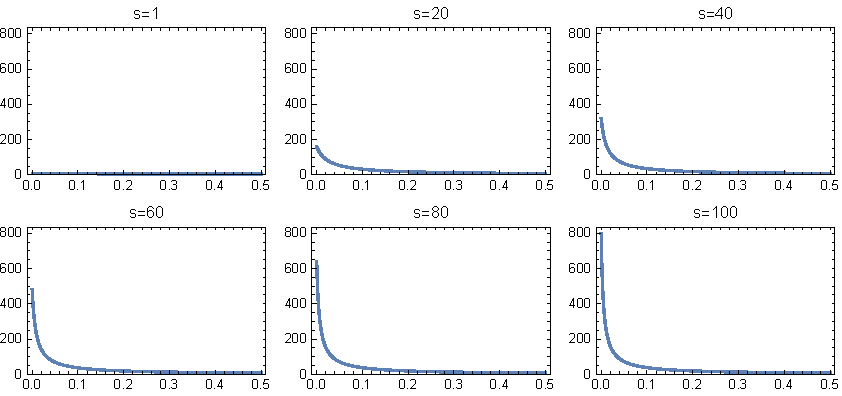
\includegraphics[width=0.45\textwidth]{plane_curvature.pdf} }}%
    \qquad
    \subfloat[Density plot of the curvature of the plane \eqref{eq_plane_curvature_evo} plotted as a function of $x$ and $y$.]{{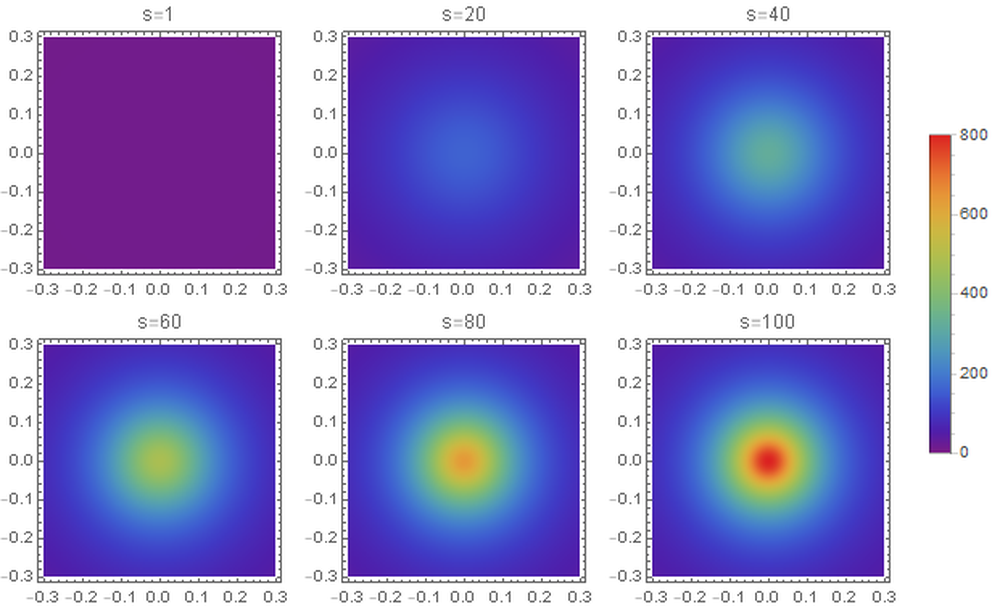
\includegraphics[width=0.45\textwidth]{sp_plane_curvature_density.png} }}%
    \label{fig:example}%
\end{figure}

\begin{figure}%
	\centering
	\subfloat[Absolute value squared of \eqref{eq_spf_plane} plotted as a function of $u$ for different values of $s$.]{{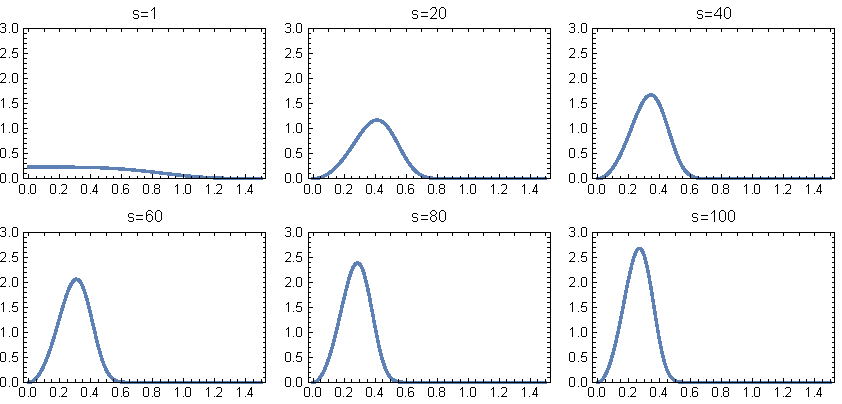
\includegraphics[width=0.45\textwidth]{sp_plane_section.pdf} }}%
    \label{fig:example}%
    \qquad
	\subfloat[Density plot of the absolute value squared of \eqref{eq_spf_plane} for different values of $s$ plotted as a function of $x$ and $y$.]{{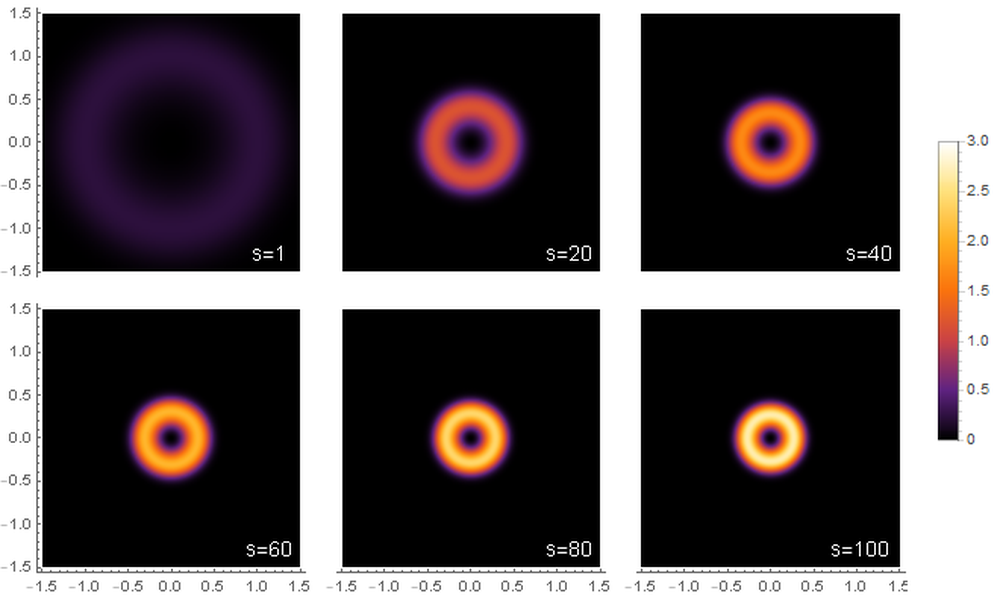
\includegraphics[width=0.45\textwidth]{sp_plane.png} }}%
\end{figure}

% The time-evolved complex coordinate is such that
% \begin{align} \label{eq_plane_normal_evolution}
% 	z_s := \left ( \phi_\tau^{X_H} \right )^* z \big|_{\tau=is} = e^{su}z
% \end{align}

We extend this to $N \in \nats$ particles. The Riemann surface representing the configuration space of the particles is the Cartesian product $(\reals^2)^N \cong \reals^{2N}$. We consider the trivial complex line bundle, $L = \reals^{2N} \times \cmplx$, with $\spot = \sum_{k=1}^{N} u_k d\theta_k$, unitary trivialization $s \equiv 1$, connection $\covd{X} = X + i \spot(X)$ and Hermitian structure $\hip{a}{b} = a \bar b$ for $a, b \in C^\infty(\reals^{2n}; \cmplx)$. The square root $\sqrtb_\pol$ of the canonical bundle is trivial with trivializing section represented by $\sqrt{dz_1 \wedge ... \wedge dz_N}$. The polarization $\pol_0$ comes from the complex structure i.e. $\overline \pol_0$ is spanned by $\{\pd{\bar z_k}\}_{k=1,...N}$ and the time-evolved polarization $\pol_\tau$ is such that $\overline \pol_\tau$ is spanned by $\{\pd{(\bar z_{s})_k}\}_{k=1,...N}$, where $(z_{s})_k = \left ( \phi_{\tau}^{X_H} \right )^* z_k \big|_{\tau=is}$ and $\bm{H} = \sum_{k=1}^{N} \frac{u_k^2}{2}$. 


%  In order to write the GCST associated to $\bm{H}$, we first determine the prequantizations and quantizations of the relevant observables. 
% \begin{equation*}
% \begin{aligned}
% \prqs_1(\bm{H}) &= \sum_{k=1}^{N} \left( - i  u_k\pd{\theta_k} - \frac{u_k^2}{2} \right), \nonumber\\
% \prqs_2(\bm{H}) &= i \sum_{k=1}^{N} \lied{\left( - u_k \pd{\theta_k} \right)}, \nonumber\\
% \end{aligned}
% \qquad
% \begin{aligned}
% \qs_1(\bm{H}) & = \sum_{k=1}^{N} -\frac{1}{2} \frac{\partial^2}{\partial \theta_k^2}, \nonumber \\
% \qs_2(\bm{H}) & = \sum_{k=1}^{N} \frac{\left( \lied{-\pd{\theta_k}}\right)^2}{2} . \nonumber
% \end{aligned}
% \end{equation*}
In this case, the GCST takes the form
\begin{align*}
	U_{s,1} = e^{\sum_{k=1}^{N} \left(- isu\pd{\theta_k} - s\frac{u_k^2}{2} \right)} \circ e^{\sum_{k=1}^{N} \frac{s}{2}\frac{\partial^2}{\partial \theta_k^2}}, \qquad U_{s,2} = e^{\sum_{k=1}^{N} i s\lied{-u \pd{\theta_k}} } \circ e^{\sum_{k=1}^{N} - i s \frac{\left( \lied{-\pd{\theta_k}}\right)^2}{2}}.
\end{align*}
The action of $U_{s,2}$ on the half-form $\sqrt{dz}$ is such that
\begin{align*}
	U_{s,2} \cdot \sqrt{dz} &= e^{i s\lied{-u \pd{\theta}} } \circ e^{- i s \frac{\left( \lied{-\pd{\theta}}\right)^2}{2}} \cdot \sqrt{dz} = \sqrt{dv + i \, d \left( 1 - i s u \pd{\theta} \right)\theta} = \sqrt{dz_{s}}.
\end{align*}
$U_{s}$ acts on the basis of wave functions describing the quantum Hall effect for one particle in the LLL as
\begin{align} \label{eq_spf_plane}
U_s(z^m e^{-\frac{\abs{z}^2}{4}} \otimes \sqrt{z}) &= e^{-\frac{m^2s}{2}}z_{s}^m e^{-\kpot_s} \otimes \sqrt{dz_s} \sim z_{s}^m e^{-\kpot_s} \otimes \sqrt{dz_s}.
\end{align}
For the integer quantum Hall effect, the result is similar. Disregarding the half-form correction in order to simplify the calculations, 
\begin{align*}
	U_{s,1} \cdot \psi_{IQHE} &\sim e^{-\frac{s}{2}} \prod_{1 \leq k<j \leq N}((z_s)_j - (z_s)_k) e^{-\kpot_s} \sim \prod_{1 \leq k<j \leq N}((z_s)_j - (z_s)_k) e^{-\kpot_s}.
\end{align*}
The Laughlin state, although similar to the IQHE state, behaves in a fundamentally different way under time-evolution. Applying the GCST, we obtain
\begin{align*} U_{s,1}(\Psi_{L}) \sim e^{-s\widehat\qs(H)} \left ( \prod_{1 \leq k < j \leq N}^N((z_{s})_j - (z_{s})_k)^m e^{-\kpot_s}\right ).
\end{align*}
The operator $e^{-s\q{H}}$ fundamentally changes the wave function. For instance, for two particles and no quasiholes, 
\begin{align*}
e^{\frac{s}{2}\left (\frac{\partial^2}{\partial \theta_1^2} + \frac{\partial^2}{\partial \theta_2^2} \right )} \cdot \left [ ((z_1)_{s} - (z_2)_{s})^3 \right ] 
= \left ( e^{-\frac{9}{2}s} (z_1)_{s}^3 - 3 e^{-\frac{5}{2}s} (z_1)^2_{s}(z_2)_{is} +  3 e^{-\frac{5}{2}s} (z_1)_{s}(z_2)^2_{s} + e^{-\frac{9}{2}s} (z_2)_{s}^3\right ).
\end{align*}
For the wave function in the presence of quasiholes, the quasihole factors also suffer a change. Indeed, a factor of $e^{-\frac{s}{2}}$ appears on the time-evolved complex variable $z_{s}$.

In the case of the Moore-Read state, by applying $e^{- \widehat \qs(H)}$, the polynomial structure becomes even less uniform than in the Laughlin state case, since some cancellation with the Pfaffian factor happens.

\subsection{Evolution on a deformed cylinder with $S^1$-symmetry} \label{sec_cyl}
Here, our Riemann surface will be the infinite cylinder $\mfld = \reals \times S^1$ with standard symplectic structure and the standard complex structure as the initial complex structure.

We consider the Kähler toric action given by a rotation of the cylinder along its axis $	\tact: S^1 \times (\reals \times S^1) \to (\reals \times S^1)$, with $\tact(e^{it}, (u,\theta)) = (u, \theta + t)$. This action has moment map $\mmap: \reals \times S^1 \to \reals$, $\mmap(u, \theta) = u$ and it is such that $\mfld^\circ = \mfld$. It is clear that $(u, \theta)$ as above define action-angle coordinates. Note that these also define a toric holomorphic chart $z = v + i\theta$ with $v = u$.

Choose the initial Kähler potential $\kpot_0 = \frac{u^2}{2}$, which coincides with the initial symplectic potential $\sgen_0$ in this case. Recalling point \eqref{intro_symplectic_evolution}, we obtain $g_{s} = \frac{u^2}{2} + sH$.

% Note also from \eqref{eq_plane_ktoric_evolution} that the action of the complex time flow on the usual complex coordinate is
% \begin{align} \label{eq_plane_normal_evolution}
% 	z_s := \left ( \phi_\tau^{X_H} \right )^* z \big|_{\tau=is} = e^{su}z
% \end{align}

Here, we consider a Hamiltonian $H \in C^\infty(\mfld)$ such that $H'' = e^{-u^2}$, i.e.
\begin{align*}
	H' = \frac{\sqrt{\pi}}{2}\erf(u), \qquad	H = \frac{1}{2}e^{- u^2} + \frac{\sqrt{\pi}}{2}u\erf{u},
\end{align*}
where $\erf(u) := \frac{2}{\sqrt{\pi}}\int_0^u e^{-t^2} dt$ is the \emph{error function}. From this and the previous considerations we obtain
\begin{align}
	\metric_s &= \left( 1 + se^{-u^2} \right) du^2 + \left( \frac{1}{1+se^{-u^2}} \right) d\theta^2, \qquad
	\kpot_s &= \frac{u^2}{2} + s (u H' - H), \qquad
	S_s &= - \left( \frac{1}{1+se^{-u^2}} \right)''. \label{eq_cyl_curvature}
\end{align}

% \begin{figure}[h]
% 	\centering
% 	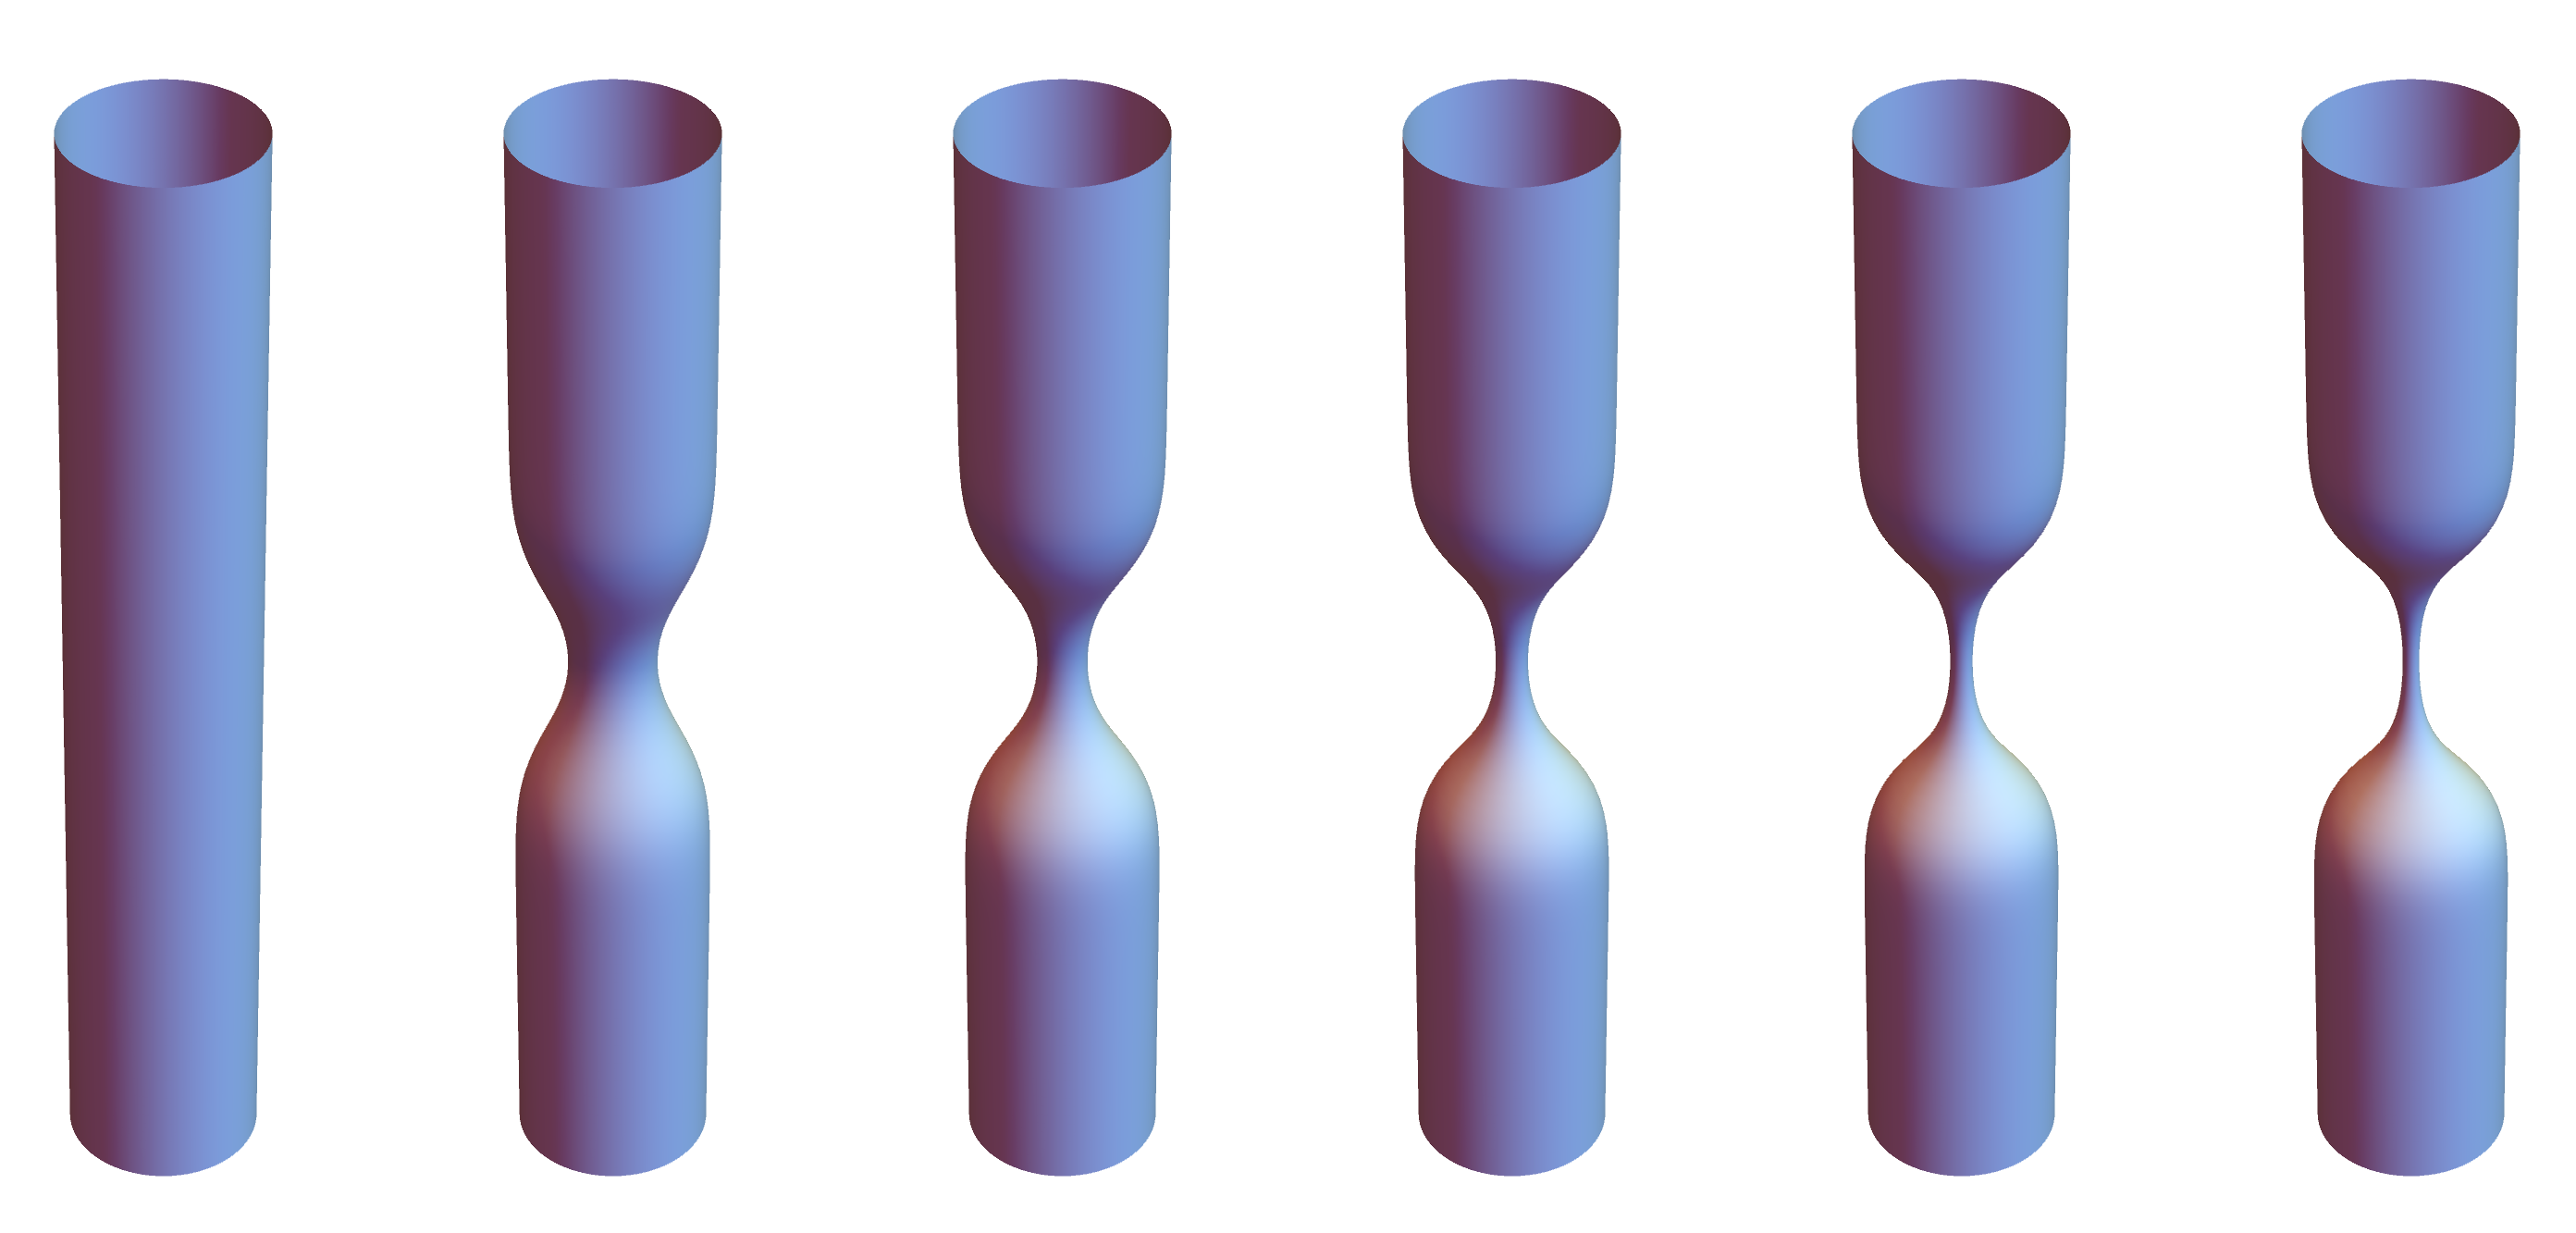
\includegraphics[width=0.5\textwidth]{cylinder_curvature_surface_isometry.png}
% 	\caption{Three dimensional illustration of the deformation that the cylinder undergoes. For visualization purpoeses, here we are rescaling the metric along the cylinder axis.}
% 	\label{fig_cylinder_curvature_illustration}
% \end{figure}

We extend this to $N \in \nats$ particles. The Riemann surface representing the configuration space of the particles will be the Cartesian product $(\reals \times S^1)^N \cong (\reals^{N} \times \torus^N)$. We consider the trivial complex line bundle, $L = (\reals^{N} \times \torus^N) \times \cmplx$, with $\spot = \sum_{k=1}^{N} u_k d\theta_k$, unitary trivialization $s \equiv 1$, connection $\covd{X} =  X + i \spot(X)$ and Hermitian structure $\hip{a}{b} = a \bar{b}$ for $a, b \in C^\infty(\reals^{N} \times \torus^N; \cmplx)$. The square root $\sqrtb_\pol$ of the canonical bundle is trivial with trivializing section represented by $\sqrt{dz_1 \wedge ... \wedge dz_N}$. The polarization $\pol_0$ comes from the complex structure i.e. $\overline \pol_0$ is spanned by $\{\pd{\bar z_k}\}_{k=1,...N}$ and the time-evolved polarization $\pol_\tau$ is such that $\overline \pol_\tau$ is spanned by $\{\pd{ (\bar z_{s})_k}\}_{k=1,...N}$, where $(z_{s})_k = \left ( \phi_{\tau}^{X_H} \right )^* z_k \big|_{\tau=is}$ and $\bm{H} = \sum_{k=1}^{N} \frac{1}{2}e^{- u_k^2} + \frac{\sqrt{\pi}}{2}u_k\erf{u_k}$. 
% In order to write the GCST associated to $\bm{H}$, we first determine the prequantizations and quantizations of the relevant observables. 
% \begin{align*}
% \begin{aligned}
% 	\prqs_1(\bm{H}) &= \sum_{k=1}^{N} - i \hbar H_k' \pd{\theta_k} - u H_k' + H_k, \\
% 	\prqs_2(\bm{H}) &= i \sum_{k=1}^{N} \lied{\left( - H_k' \pd{\theta_k} \right)}, \nonumber\\
% 	\qs_1(\bm{H}) &= \sum_{k=1}^{N} H_k \left (- i \pd{\theta_k} \right ), \nonumber
% \end{aligned}
% \qquad
% \begin{aligned}
% 	\qs_2(\bm{H}) &= \sum_{k=1}^{N} H_k \left (\lied{-\pd{\theta_k}} \right ) . \nonumber \\
% 	U_{s,1} &=  e^{ \sum_{k=1}^{N} -siH_k'\pd{\theta_k}-suH_k'+sH_k} e^{ \sum_{k=1}^{N} -sH_k(-i  \pd{\theta_k})}, \\
% 	U_{s,2} &=  e^{i \sum_{k=1}^{N} \lied{\left( - u_k \pd{\theta_k} \right)}}. % e^{ \sum_{k=1}^{N} H_k \left (\lied{-\pd{\theta_k}} \right )}
% \end{aligned}
% \end{align*}
We will work with adaptations of the quantum Hall states for the cylinder given in \cite{azuma_explicit_1994}. For the case of the plane, the wave function for one particle in the LLL takes the form
\begin{align*}
	\psi_{m} \sim \tilde \psi_m \otimes \sqrt{dz}, \qquad \tilde \psi_{m} \sim w^m e^{-\kpot_0} = e^{2 \pi m (u + i\theta)} e^{-\frac{u^2}{2}}, \qquad w = e^{m 2\pi (u+i\theta)}.
\end{align*}
Applying the GCST, we obtain
\begin{align}\label{eq_cyl_spf_evolution}
	U_{s,1} \tilde \psi_m &= e^{-s H \left (\frac{2 \pi}{L_\theta} m \right )} w_s e^{-\kpot_s}, \qquad w_s = e^{2\pi \left (v_s + i \theta_k \right )}, \\
	U_{s,2} \cdot \sqrt{z} &= e^{i s\lied{-u \pd{\theta}} } \cdot \sqrt{z} = \sqrt{dv + i \, d \left( 1 - i s H' \pd{\theta} \right)\theta}= \sqrt{dz_{s}}.
\end{align}

\begin{figure}%
	\centering
	\subfloat[Curvature of cylinder \eqref{eq_cyl_curvature} plotted as a function of $u$.]{{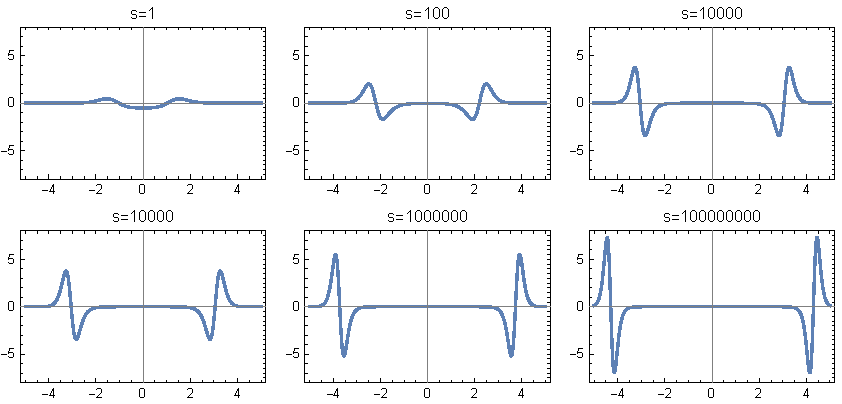
\includegraphics[width=0.45\textwidth]{cylinder_curvature.pdf} }}%
	\qquad
	\subfloat[Density plot of the curvature of the cylinder \eqref{eq_cyl_curvature} in three dimensions, for the same values of $s$ as the left figure.]{{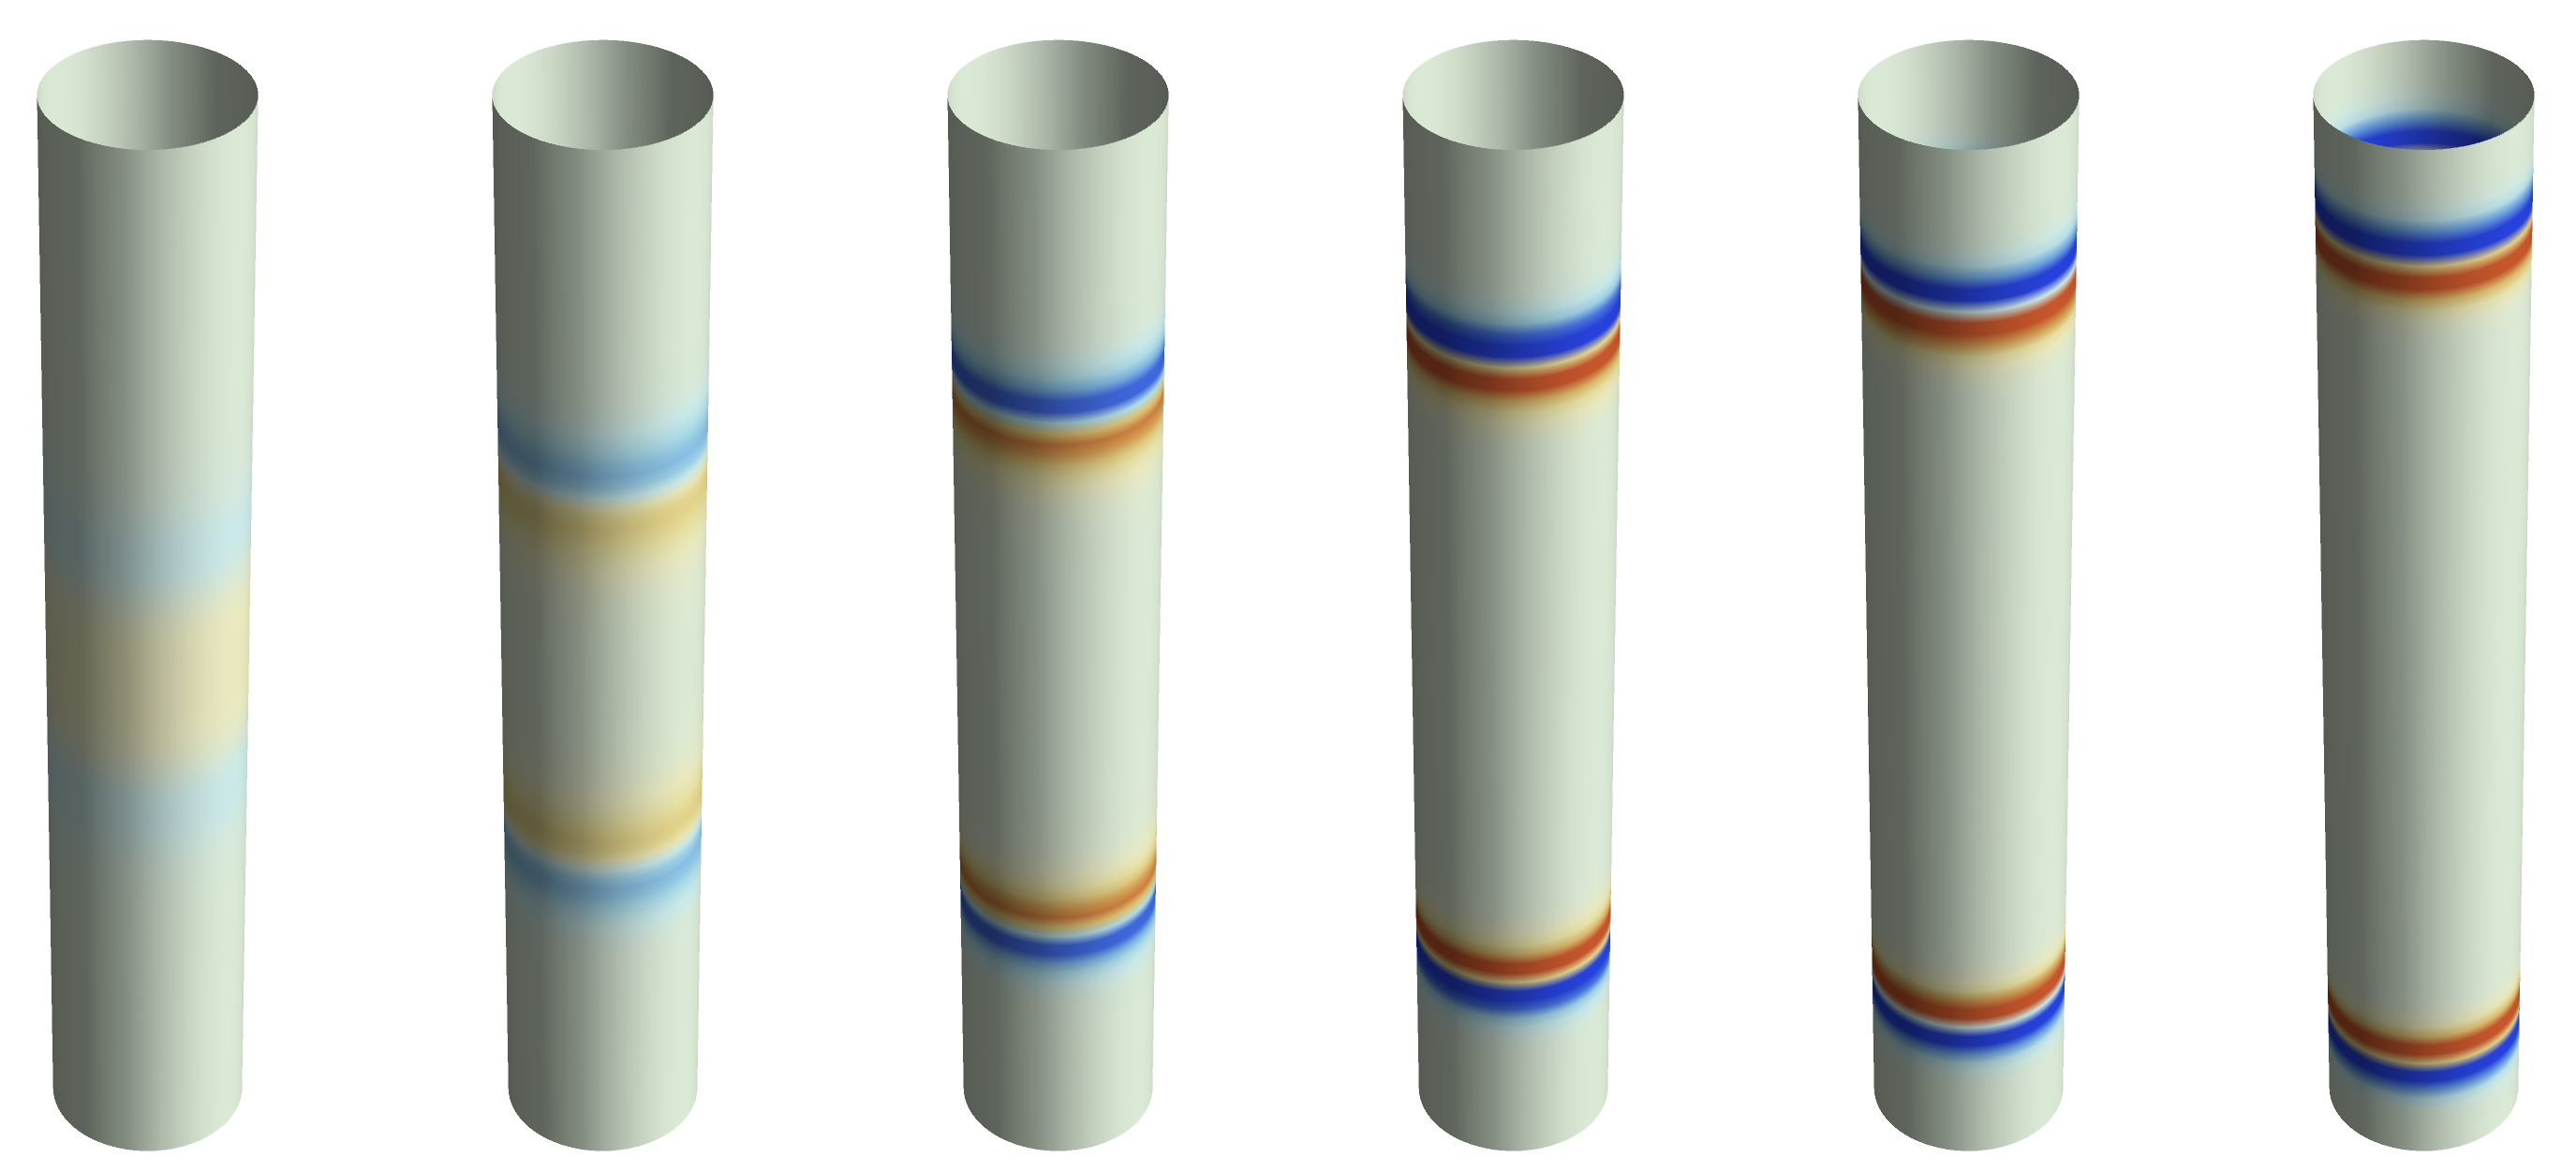
\includegraphics[width=0.45\textwidth]{cylinder_curvature_surface.png} }}%
    \label{fig:example}%
\end{figure}

\begin{figure}%
	\centering
	\subfloat[Density plot of the absolute value squared of \eqref{eq_cyl_spf_evolution} plotted as a function of $u$ for different values of $s$.]{{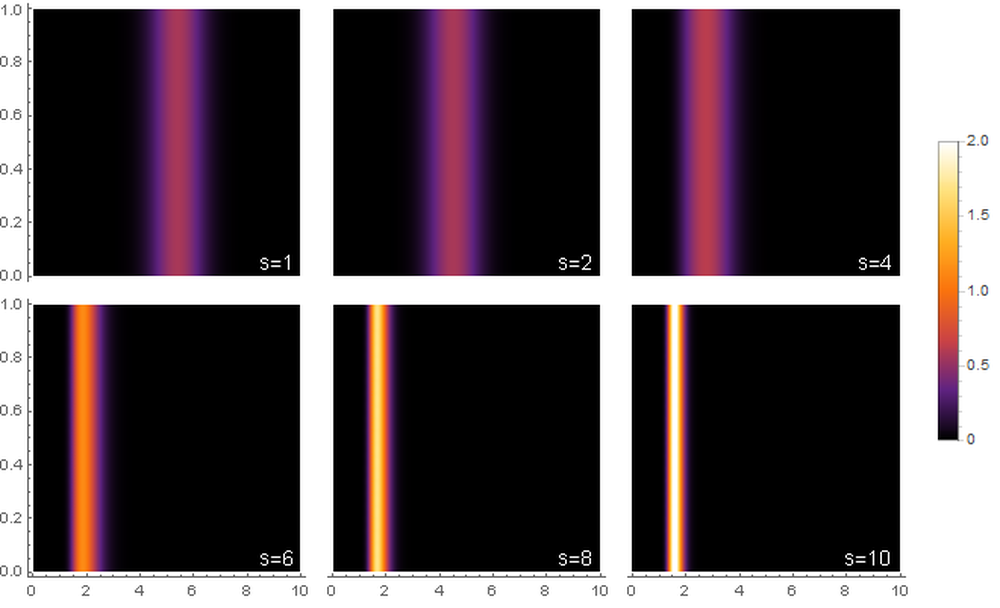
\includegraphics[width=0.45\textwidth]{sp_cyl.png} }}%
	\qquad
	\subfloat[Absolute value squared of \eqref{eq_cyl_spf_evolution} plotted as a function of $u$ for different values of $s$.]{{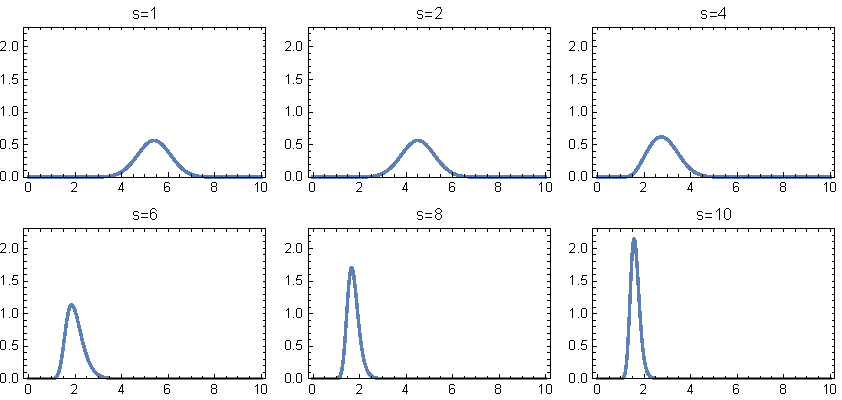
\includegraphics[width=0.45\textwidth]{sp_cyl_section.pdf} }}%
    \label{fig:example}%
\end{figure}

In order to simplify the calculations, we will not consider the half-form correction in the remainder of this section. The wave function for the fully filled LLL is
\begin{align*}
	\psi_\text{IQHE} = \prod_{1 \leq k < j \leq N}(w_j-w_k) e^{-\sum_{k}^N\frac{u_k^2}{2}} &= \prod_{1 \leq k < j \leq N}\left(e^{2\pi (u_j + i \theta_j)}-e^{2\pi (u_k + i \theta_k)}\right) e^{-\sum_{k}^N\frac{u_k^2}{2}},
\end{align*}
where $w_k = e^{\frac{2\pi (u_k+i\theta_k)}{L_x}}$. Applying the GCST, we obtain
\begin{align} \label{eq_cyl_iqh_evolution}
	U_{s,1} \psi_\text{IQHE} &= \prod_{1 \leq k < j \leq N}((w_j)_s-(w_k)_s) e^{-\kpot_s}, \qquad (w_k)_s = e^{2\pi \left ((v_k)_s + i \theta_k \right )}. \\
	U_{s,1} \psi_\text{L} &= e^{- s \sum_{k=1}^{N} H_k \left (- i \pd{\theta} \right )} \cdot \left ( \prod_{1 \leq k < j \leq N}(w_j-w_k)^m e^{\left( -\sum_{k}\frac{u_k^2}{2}\right)} \right )
\end{align}
As for the Laughlin wave function in the case of the cylinder, the structure of the holomorphic factor of the wave function is fundamentally changed as in the case of the plane.

Noting that $\lim_{s \to \infty} \pol_s =  \langle X_u \rangle = \left \langle \pd{\theta} \right \rangle$ and adapting the proof of Lemma 3.7 of \cite{baier_toric_2011}, we obtain in the case of a single particle wave function in the LLL that 
\begin{align*} \label{eq_cyl_limit}
	\tilde \psi_m &= \xrightarrow{s\to\infty} ~ \delta(u-2\pi m) e^{2 \pi m + 2 \pi m i \theta} \sqrt{H''(2\pi m)}\sqrt{du}, \nonumber
\end{align*}
yielding a distributional wave function.


% \subsection{Deformed torus}
% \cite{gradshtein_table_2007} odd theta function
% \begin{align*}
% 	z_{it} &= e^{itX_f}z = x+itf'(y)+iy \\
% 	&= x+i(y+tf'(y))
% \end{align*}
% \begin{align*}
% 	\vartheta(z) = \frac{1}{i}\sum_{n=-\infty}^{\infty}(-1)^n q^{\left(n+\frac{1}{2}\right)^2}e^{(2n+1)zi} = 2\sum_{n=1}^{\infty}(-1)^{n+1}q^{\left(n-\frac{1}{2}\right)^2}\sin[(2n-1)z]
% \end{align*}
% $q=e^{i\pi\tau}$
% wave function \cite{haldane_periodic_1985}
% \begin{align*}
% 	\psi(x,y) &= e^{ikz} e^{-\frac{y^2}{2}} \prod_{\nu=1}^{N}\vartheta\left(  \frac{\pi(z-z_\nu)}{L_1}\Big|\tau\right) \\
% 	&= 2 e^{ikz} e^{-\frac{y^2}{2}} \prod_{\nu=1}^{N} \sum_{n=1}^{\infty}(-1)^{n+1}e^{i\pi\tau\left(n-\frac{1}{2}\right)^2}\sin\left[(2n-1)\frac{\pi(z-z_\nu)}{L_1}\right] 
% \end{align*}
% From \cite{jain_composite_2007}
% \begin{align*}
% 	\psi_{k_x}=\sum_{n=-\infty}^{\infty}e^{-\frac{1}{2}(y-nL_y-k_x)^2}e^{i(k_x+nL_y)x}
% \end{align*}
% with Kähler potential
% \begin{align*}
% 	\psi_{k_x}=e^{-\frac{y^2}{2}}\sum_{n=-\infty}^{\infty}e^{-\frac{1}{2}(y-nL_y-k_x)^2}e^{i(k_x+nL_y)x}=\sum_{n=-\infty}^{\infty}e^{-\frac{1}{2}\left[y^2 + (y-nL_y-k_x)^2 \right]}e^{i(k_x+nL_y)x}
% \end{align*}
% \begin{align*}
% 	H_k(y) &= \frac{\sin(2\pi ky)}{(2\pi k)^2} \\
% 	H'_k(y) &= \frac{\cos(2\pi ky)}{2\pi k} \\
% 	H_k'' &= - \sin(2 \pi k y)
% \end{align*}
% \matosc{
% \[
% 	(u,\theta) \sim (v,\theta)
% \]}


% %_______
% \begin{align*}
% 	X_H &= - H'(y)\pd{x} \\
% 	\prq{H} &= - i \hbar X_H - \spot(X_H) + H \\
% 	\spot &= -y dx \\
% 	\prq{H} &= i \hbar H'(y) \pd{x} - y H'(y) + H = i \hbar \frac{\cos(2\pi ky)}{2\pi k} \pd{x} - \left( y \frac{\cos(2\pi k y)}{2\pi k} - \frac{\sin(2\pi k y)}{(2\pi k^2)} \right)\\
% 	\q{H} &= H(\prq{y}) \\
% 	X_y &= - \pd{x} \\
% 	\prq{y} &= i \hbar \pd{x} \\
% 	\q{H} &= H(i \hbar \pd{x}) = \frac{\sin(2\pi i \hbar k \pd{x})}{(2\pi k)^2} \\
% 	U_{is} &= e^{\frac{s}{\hbar}\prq{H}}\circ e^{-\frac{s}{\hbar}\q{H}} \\
% 	&= e^{siH'(y)\pd{x}-\frac{sy}{\hbar}H'(y)+\frac{s}{\hbar}H}\circ e^{-\frac{s}{\hbar}H(i \hbar \pd{x})} \\
% 	&= e^{i s \frac{\cos(2\pi ky)}{2\pi k} \pd{x} - \frac{s}{\hbar} \left( y \frac{\cos(2\pi k y)}{2\pi k} - \frac{\sin(2\pi k y)}{(2\pi k^2)} \right)}e^{- \frac{s}{\hbar}\frac{\sin(2\pi i k \pd{x})}{(2\pi k)^2}} \\
% 	s_n &=  \\
% 	U_{is} s_n &= 
% \end{align*}
% \begin{align*}
% 	e^{\pd{y}} \psi = e^{\pd{y}}\sum_{n=-\infty}^{\infty}e^{-\frac{1}{2}\left[y^2 + (y-nL_y-k_x)^2 \right]}e^{(k_x+nL_y)x} = 
% \end{align*}
%-------
\end{document}